\chapter{ RÉALISATION }

        \section{Classes métier}
        Dans cette partie, nous allons décrire les classes les plus importantes dans le fonctionnement de l'application. Nous ne mentionnerons également que les méthodes les plus importantes de chaque classe.
        \begin{itemize}
        \vspace{0.2cm}
            \item \textbf{Client :} Cette classe permet de communiquer avec le serveur, elle est utile notamment pour l'inscription et la connexion au réseau Evernet. 
            \begin{lstlisting}[language = Java , frame = trBL , firstnumber = last , escapeinside={(*@}{@*)}]
            // Methodes de requetes serveur
            String signIn()
            HashMap<String, String> logIn()
            HashMap<String, String> getPhoneNb()
            HashMap<String,String> getPhoneNumList()
            String getInvitationKey()
            ArrayList<String> getAllAlias()
            
            // Communication
            openSocket()
            closeSocket()
            sendDataToServer()
            String receiveDataFromServer()
            
            // Parsing de donnees
            String truncateMarkers()
            String addMarkers()
            \end{lstlisting}
            
           \vspace{0.2cm}
            \item \textbf{Contact :} La classe Contact contient les informations des utilisateurs (nom et identifiant). Cette classe est Parcelable afin de permettre le passage d'un ArrayList d'objets de type Contact entre deux activités.
            \begin{lstlisting}[language = Java , frame = trBL , firstnumber = last , escapeinside={(*@}{@*)}]
            public void writeToParcel(Parcel dest, int flags);
            public Contact[] newArray(int size);
            
            \end{lstlisting}
            
             
            \item \textbf{Handler :} La classe Handler enregistre les différentes images (ReceivedFile) qu'elle reçoit.
            \vspace{0.2cm}
            
            \item \textbf{ContactAdapter :} Cette classe hérite de la classe BaseAdapter, elle a été conçue pour proposer un Adapter pouvant utilisée des objets de type Contact. Elle est utilisée dans la classe DisplayContact comme Adapter pour la Listview affichant les contacts à l'utilisateur.
            \vspace{0.4cm}
            
            \item \textbf{Packet :} la classe Packet décrit le format d'un paquet et permet de gérer les différents champs de ce dernier.
            \begin{lstlisting}[language = Java , frame = trBL , firstnumber = last , escapeinside={(*@}{@*)}]
            // Extraction des champs du paquet
             String extractSrc()
             String extractDst()
             String extractPosition()
             String extractNBpackets()
             String extractNameOfIm()
             String extractTtl()
             String extractFragment()
            \end{lstlisting}
            \vspace{0.2cm}
            
            \item \textbf{ReadWriteFile :}
            La classe ReadWriteFile permet l'écriture et la lecture de fichiers sur nos smartphones Android. Elle est principalement utilisée pour l'écriture et la lecture des certificats.
             \begin{lstlisting}[language = Java , frame = trBL , firstnumber = last , escapeinside={(*@}{@*)}]
            String readFromFile()
            String writeToFile()
            \end{lstlisting}
            \vspace{0.2cm}
            
            \item \textbf{SmsReceiver :} Cette classe permet de recevoir les SMS et les traiter en utilisant les classes Handler et ReceivedFile.
            \vspace{0.2cm}
           
            \begin{lstlisting}[language = Java , frame = trBL , firstnumber = last , escapeinside={(*@}{@*)}]     
            public View getView(int position, View convertView, ViewGroup parent)
            \end{lstlisting}
            \vspace{0.2cm}
            
            \item \textbf{FileManager :} Elle permet de compresser l'image et de la découper en fragments.
            \begin{lstlisting}[language = Java , frame = trBL , firstnumber = last , escapeinside={(*@}{@*)}]
            // Recupere une image stockee sur le telephone
            // et renvoie une bitmap compressee de l'image
            Bitmap getResizedBitmap()
            
            // Converti un entier en string et ajoute du bourrage si necessaire
            String intToString()
            
            // Recuperation du prochain fragment d'image donnee en String
            String getNextFragment()
            \end{lstlisting}
            \vspace{0.2cm}
            
            \item \textbf{ReceivedFile :} Elle permet à la réception, de regrouper les paquets ayant le même expéditeur et appartenant à la même image d'origine.\\
            Une fois que tous les paquets attendus sont reçus, elle concatène les fragments des paquets.  
            
            \begin{lstlisting}[language = Java , frame = trBL , firstnumber = last , escapeinside={(*@}{@*)}]
            insertPacket()
            
            // Conversion
            byte [] stringToArrayBytes()
            Bitmap byteArrayToBitmap()
            String toImageString()
            
            \end{lstlisting}
        \end{itemize}
        
        \section{Entête du paquet SMS }\label{epSMS}
        Pour fabriquer le paquet sms, nous nous sommes inspirés du format des paquets IP. Il comprend des champs qui permettent d'identifier sa source, sa destination, le fragment de l'image à envoyer, et d'autres éléments permettant la reconstruction de l'image à la réception des paquets. Les paquets ont le format ci-dessous : 
        
        \begin{table}[htbp]
          \begin{tabular}{|c|*{6}{c|}}
             \hline
             Source & Destination & Position & Nombre de paquets & Horodatage & TTL & Fragment  \\
             \hline
        \end{tabular} \\
        <--10---><------10-----><---8----><---------4--------------><-------6------><--1--><-------------
            \caption{Format d'un Paquet SMS}
            \label{tab:my_label}
        \end{table}
        
        \begin{itemize}
            \item \textbf{Source :} Correspond au pseudonyme  de l'expéditeur de l'image. Sa longueur est de dix caractères. \\
            \item \textbf{Destination :} Correspond au pseudonyme du destinataire final de l'image. Comme la source, la taille du champ destination est exactement de dix caractères. \\
            \item \textbf{Position :} C'est un tableau d'entiers qui correspond aux positions des fragments sur le nombre total de paquets. cette information permet d'ordonner les paquets à la réception.\\
            Le nombre de fragments contenus dans le paquet (c'est à dire ceux qui sont XOr) est égal au nombre d'entiers du tableau différents de zéro.\\
            \item \textbf{Nombre de paquets :} Ce champ correspond au nombre total de paquets obtenu après le découpage de l'image. Il permet de vérifier à chaque réception de paquet, si la totalité des paquets attendus a été reçu en comparant ce champs au nombre de paquets reçus.\\
            
            \item \textbf{Horodatage(timeStamp) :} Correspond à l'heure à laquelle l'image à envoyer a été découpée en fragments. Ce champ permet à la réception, d'éviter de mélanger des paquets qui, bien qu'ils proviennent de la même source, n'appartiendraient pas à la même image. Par exemple, un utilisateur peut envoyer simultanément deux images à quelqu'un, dans la mesure où les paquets empruntent différents chemins qui peuvent être plus ou moins  rapides. Un paquet de la seconde image peut arriver avant un paquet de la première. Dans ce cas, l'heure de découpage est le moyen que nous avons trouvé pour palier ce problème.\\
            Une image sélectionnée, découpée à 18heure 25 minutes 2 secondes aura pour timeStamp 182502. Cette technique a malgré tout sa limite. Par exemple un utilisateur envoie avec un téléphone tellement performant qu'il soit capable de sélectionner, découper, et envoyer les paquets de deux images différents dans un même temps. Un exemple typique serait que l'utilisateur découpe l'image nommée "A" à 18h25min02s et envoie tous les paquets, puis reprend la même procédure avec une deuxième image nommée "B" et qu'il soit toujours 18h25min02. Mais la probabilité que ce phénomène se produise est sensiblement très faible. Premièrement, nous n'avons pas parallélisé ces étapes, deuxièmement le nombre d'opérations qui s'effectuent dans les algorithmes de la sélection de l'image à l'envoi total des paquets est aussi grand.\\
            
            \item \textbf{TTL :} Comme pour les paquets IPs, ce champ correspond à la durée de vie d'un paquet. Il indique par combien d'intermédiaires le paquet pourra transiter avant qu'il arrive soit à la destination, ou qu'il soit détruit. C'est un entier qui se décrémente d'une unité à chaque intermédiaire.
            
            Dans notre projet, nous avons fixé sa valeur maximale à 9. Donc son champ occupe un caractère.\\
            \item \textbf{Fragment :} Fragment de l'image à envoyer. Comme indiqué dans la section ~\ref{decoupage}, la contrainte de la longueur maximale de caractères qui peuvent être envoyés d'un seul coup, nous oblige à limiter la longueur maximale d'un fragment à 100 caractères.
        \end{itemize} 
        
        
        \section{Algorithmes et méthodes}
         \subsection{Découpage de l'image}\label{decoupage}
        L'image à découper est transformée en tableau de pixels (bitmap), puis en tableau de bytes. 
        Les données à envoyer par SMS étant des chaînes de caractères, nous avons donc transformé ce tableau de bytes en une longue chaîne de caractères que nous avons par la suite découpée en petits fragments de chaînes de caractères de taille maximale 100. \\
        La longueur maximale d'un SMS ( paquet SMS dans ce projet) qui peut être envoyé d'un seul coup est de 160 caractères. Cette contrainte influe directement sur la longueur maximale des fragments de l'image et nous avons donc dû, pour faire de la place aux autres champs  de l'en-tête du paquet, limiter à 100 caractères la taille maximale d'un fragment.
        
        
        \paragraph{}
          Dans les champs source et destinataire, lorsque la longueur du pseudo est inférieure à 10, nous effectuons un bourrage avec le caractère "*".  Par exemple, le pseudo "Bob" devient "*******Bob" après bourrage.
          De même pour les paramètres position et nombre de paquets qui sont des entiers, nous bourrons avec des 0 au début. par exemple 3 et 15 deviennent respectivement 0003, 0015.
         \begin{lstlisting}[language = Java , frame = trBL , firstnumber = last , escapeinside={(*@}{@*)}]
         public Bitmap getResizedBitmap(ContentResolver cr, Uri u) throws IOException {
            originalImage = MediaStore.Images.Media.getBitmap(cr,u);

            width = originalImage.getWidth();

            height = originalImage.getHeight();
            matrix = new Matrix();
            scaleWidth = ((float) newWidth) / width;
            scaleHeight = ((float) newHeight) / height;
            matrix.postScale(scaleWidth, scaleHeight);
            resizedBitmap = Bitmap.createBitmap(originalImage, 0, 0, width, height, matrix, true);

            outputStream = new ByteArrayOutputStream();
            resizedBitmap.compress(Bitmap.CompressFormat.JPEG, 10, outputStream);
            imageBytes = outputStream.toByteArray();
            newWidth = resizedBitmap.getWidth();
            newHeight = resizedBitmap.getHeight();
            imageString = Base64.encodeToString(this.imageBytes, Base64.DEFAULT);
            Date currentTime = Calendar.getInstance().getTime();
            int heure = currentTime.getHours();
            int min = currentTime.getMinutes();
            int sec = currentTime.getSeconds();
            this.imageName = intToString(heure) + intToString(min) + intToString(sec);
         return resizedBitmap;
        }
        \end{lstlisting}
        %donner un exemple avec un shcema mettre la taille et le format des paquets
        
        \subsection{Gestion des paquets  par les noeuds à la réception}
        
        Lorsqu'un utilisateur reçoit un paquet, il vérifie dans l'en-tête s'il est le destinataire.\\
        \begin{itemize}
            \item  Si oui, alors il regarde dans sa hashmap s'il a déjà reçu des paquets du même expéditeur avec le même horodatage (timestamp). 
            \begin{itemize}
                     \item Si c'est le cas, alors il insère le paquet dans cette liste s'il n'y est pas.
                     \item Sinon il crée une nouvelle liste et l'insère pour dire que c'est le début d'une nouvelle image.
            \end{itemize}
            \item Sinon cela veut dire que ce paquet doit être transféré vers d'autres destinataires.
            Avant le transfert, il doit d'abord vérifier le TTL. S'il est supérieur à 1, alors il est décrémenté de 1, puis le paquet renvoyer à d'autres destinataires sélectionnés depuis le serveur. Nous avons implémenté deux versions dans le cas où le TTL est inférieur à 1 :
            \begin{itemize}
                \item On jette le paquet.
                \item On transfère le paquet directement à sa destination.
            \end{itemize}
        \end{itemize}
        La première version marcherait si le réseau était petit comme celui sur lequel nous réalisons les tests. Cependant, plus le réseau grandit, plus la probabilité que le destinataire finale fasse partie de la liste des prochains destinataires tirés du serveur devient petit. Donc, il se peut qu'aucun paquet n'arrive à destination.
        Finalement, nous avons gardé la deuxième version qui garanti l'envoi à la destination. \\
        
        La requête au serveur pour obtenir des destinataires intermédiaires ne renvoie rien si l'utilisateur a été déconnecté du serveur, donc pas authentifié. Dans ce cas, il doit se reconnecter et s'authentifier à nouveau avant de réessayer la requête. Si l'opération échoue toujours, alors le paquet est jeté.
        
        \begin{lstlisting}[language = Java , frame = trBL , firstnumber = last , escapeinside={(*@}{@*)},caption = Dans SmsReceiver]

    public void setPacketInHandler(Context context, String stringPack) {

        Packet packet=new Packet();
        packet.setPacket(stringPack);
        ReceivedFile file;
        String key=packet.getSource()+packet.getDestination()+packet.getTimeStamp();
        String myPhoneNumber=getDefaults(PHONE_NUMBER,context);
        if(packet.getDestination().equals(myPhoneNumber)) {
            boolean contains = handler.contains(key);
            if (contains==false) {
                file = new ReceivedFile(key);
                file.insertPacket(packet.getPosition(),packet.getImageFragment());
                file.setNbPackets(packet.getNbPackets());
                handler.insertFile(key,file);
            } else {
                file=handler.getFileByKey(key);
                file.insertPacket(packet.getPosition(),packet.getImageFragment());
            }
            Toast.makeText(context,"message :" + file.getSize(), Toast.LENGTH_LONG).show();
            this.imageView(context, file, key);
        } else {
            dashboardActivity = DashboardActivity.instance();
            packet.decreaseTTL();
            String target=null;
            if( packet.getTtl() <=1 ) {
                target= packet.getDestination();
            }
            dashboardActivity.sendTo(packet.getPacket(),target);
        }
    }

    \end{lstlisting}
          
         \subsection{Reconstitution et stockage de l'image à partir des paquets reçu}
         Après insertion d'un paquet, l'algorithme vérifie si tous les paquets attendus ont été reçus, en comparant le champ "Nombre de paquets" à la taille de la liste. Si les deux sont égaux, alors tous les paquets ont été reçus et dans ce cas on peut reconstruire l'image. 
        
        La reconstruction est l'opération inverse du découpage. On extrait le fragment d'image dans chaque paquet selon l'ordre croissant des numéros des paquets (de 0 à Nombre de paquets - 1), puis on concatène ces fragments pour former une longue chaîne de caractères.\\
        
        Cette chaîne  est ensuite transformée  en un tableau de bytes (arrayBytes) et enfin tableau de pixels(bitmap). L'utilisateur recevra une notification "Image reçue". \\
         Pour l'instant nous sauvegardons les images que nous recevons de l'application dans la galerie, dans un dossier appelé "Pictures" avec comme nom PSEUDO + timestamp. Les images dans ce dossier se classent de la plus récente à la plus anciennement reçue. Ce qui permet à l'utilisateur de retrouver plus facilement les images reçue tout dernièrement.\\
       
       \begin{lstlisting}[language = Java,frame = trBL , firstnumber = last , escapeinside={(*@}{@*)}, caption=Dans SmsReceiver.java ]
            public void imageView(Context context, ReceivedFile file, String key) {

                if(file.allPacketReceived()) {
                        byte [] bytes = file.stringToArrayBytes();
                        Toast.makeText(context,"Image recue :" + bytes.length, Toast.LENGTH_LONG).show();
                        Bitmap bitmap = file.byteArrayToBitmap(bytes);
                        MediaStore.Images.Media.insertImage(context.getContentResolver(), bitmap, key, "EvernetImage");
                }
            }
       \end{lstlisting}
      
        \subsection{Network Coding Topologie}
        
            Dans un premier temps et dans le but d'avancer dans le projet, nous a décidé de fixer la topologie dans laquelle s'insère le Network Coding, et pour cela, on l'a adaptée pour avoir une destination, une source et quatre nœuds intermédiaires. D’abord, la topologie est fixée dans la source après avoir demandé au serveur quatre nœuds intermédiaires. Ensuite, la topologie sera envoyée au serveur pour qu’elle soit exploitée quand un nœud intermédiaire demande une liste de destinataires. Quand un nœud intermédiaire reçoit deux paquets différents et c’est lui le responsable de l’encodage, il encode immédiatement, ce sont deux derniers et il envoie le paquet encoder à son voisin renvoyé par le serveur. Enfin, une fois que la destination a reçu tous les paquets soit encodée ou non elle procède pour le décodage des paquets encodés en utilisant les paquets en clair (non chiffrés).
        
        \begin{figure}[H]
                \centering
                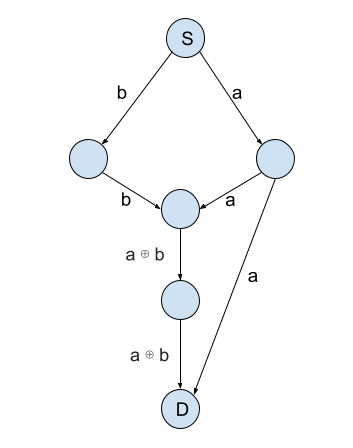
\includegraphics[scale=0.5]{images/NC_topology.png}
                \caption{Topologie Network Coding réaliser}
                \label{fig:Network_Coding_Topologie}
        \end{figure}
        
        \subsection{Network Coding implémentation}
        
        \paragraph{} Le Network Coding est un point capital de cette application. Cette notion de Network Coding étant nouvelle, nous avons pris du temps pour effectuer des recherches et comprendre comment l'appliquer dans notre projet. La difficulté ici est la particularité du réseau. En effet dans les exemple que l'on a pu voir au sujet du Network Coding, les noeuds du réseau peuvent physiquement communiquer avec leurs voisins.
        Le réseau sur lequel nous travaillons n'ayant pas de voisin physique, fixer une topologie comme celle vue précédemment est nécessaire.
        Une nécessité que nous n'avons compris que très tard. Cela a fortement impacté l'avancement de notre projet.\\
        Nous avons essayé d'implémenter deux versions du Network Coding. À ce jour aucune de ces implémentations n'a pu êtres testées.
        
        
        \subsubsection{Implémentation élimination de Gauss-Jordan}
        
        \paragraph{}La première implémentation consiste à encoder les fragments des paquets en une combinaison linéaire.
        Une combinaison linéaire de la forme : \textbf{Ax + By}, \textbf{A} et \textbf{B} étant les fragments et \textbf{x}, \textbf{y} leurs coefficients respectifs.
        Le nouveau fragment créé est ainsi envoyé au noeud suivant pour y être combiné à nouveau dans le cas d'un noeud intermédiaire, ou bien d'être décodé s'il s'agit de la destination.
        
        \paragraph{}Il existe plusieurs méthodes pour résoudre un système d'équations linéaires.\\
        Dans le cas du Network Coding la solution la plus adaptée est l'élimination de Gauss-Jordan. 
        Pour ce faire on crée une matrice de taille n*n, "n" étant le nombre de fragment d'une image. 
        On a donc chaque colonne de la matrice qui correspond à un fragment de l'image.
        Chaque ligne de la matrice correspondant à une combinaison linéaire de ces fragments.
        Les nombres dans la matrice représentent donc les coefficients attribués aux fragments dans les combinaisons linéaires.
        En parallèle on construit un vecteur colonne de taille n, avec les valeurs des fragments en faisant correspondre les valeurs des lignes du vecteur avec les combinaisons des lignes de la matrice.
        Pour simplifier le développement nous nous sommes appuyés sur une la librairie \textbf{"la4j"}\cite{la4j}.
        Cette librairie dispose d'une fonction solve().
        Cette fonction est appelée sur la matrice précédemment créée en passant en argument le vecteur colonne contenant les valeurs de fragments.\\
        Nous avons cependant rencontré un problème au niveau des types entre les valeurs des paquets qui sont de type "long" et les valeurs dans la matrice qui sont elles des "double".
        La conversion "long" vers "double" fait perdre des chiffres, ce qui fausse la résolution du système d'équation. 
        On obtient donc un résultat erroné.\\
        
        \paragraph{}Pour résoudre ce problème il faudrait écrire des fonctions adapté à notre format. La Dead-Line se rapprochant nous avons choisi d'implémenter une version simple de Network Coding. Cela afin d'avoir un modèle à présenter.
        
        \subsubsection{Implémentation XOR}
        
        L'utilisation du XOR pour le Network Coding permet de visualiser de façon simple le but et l'intérêt du NC.
        Dans la topologie vu précédemment sur le schéma figure : \ref{fig:Network_Coding_Topologie}  , si un paquet arrive sur un noeud relais alors celui-ci l'encode avec le prochain paquet de la même image qu'il recevra.\\
        Quand un appareil reçoit un paquet encodé, il regarde s'il peut le décoder avec les paquets déjà reçus.
        Si ce n'est pas possible il le stock pour le déchiffré si possible avec le prochain paquet reçus.
        L'encodage et le décodage se font à l'aide de l'opération binaire XOR.\\
        
        Fonction d'encodage des fragments :
        
        \begin{lstlisting}[language = Java , frame = trBL , firstnumber = last , escapeinside={(*@}{@*)}]
        
        static public Packet mergeTwoPackets(Packet firstPacket, Packet secondPacket){

            String firstPacketFragment = firstPacket.getImageFragment();
            String secondPacketFragemnt =  secondPacket.getImageFragment();
    
            int[] firstPacketPos = firstPacket.getPosition();
            int[] secondPacketPos = secondPacket.getPosition();
    
            int[] mergePacketPos = {firstPacketPos[0],secondPacketPos[0]};
    
            byte[] firstPacketFragmentBytes = firstPacketFragment.getBytes();
            byte[] secondPacketFragmentBytes = secondPacketFragemnt.getBytes();
    
            byte[] mergedPacketsFragmentBytes = new byte[firstPacketFragmentBytes.length];
    
            for (int i=0; i < mergedPacketsFragmentBytes.length; i++){
                mergedPacketsFragmentBytes[i] = (byte) (firstPacketFragmentBytes[i] ^ secondPacketFragmentBytes[i]);
            }
    
            String mergedPacketsFragment = new String(mergedPacketsFragmentBytes);
    
    
    
            Packet output = new Packet(firstPacket.getSource(),
                    firstPacket.getDestination(),
                    mergePacketPos,
                    firstPacket.getNbPackets(),
                    firstPacket.getTtl(),
                    firstPacket.getTimeStamp(),
                    mergedPacketsFragment);
            return output;
        }
        
        \end{lstlisting}
        \\
        
        Fonction de décodage des des Fragments :
        
        \begin{lstlisting}[language = Java , frame = trBL , firstnumber = last , escapeinside={(*@}{@*)}]
        
        static public Packet decodeMergedPacketWithOnePacket(Packet mergedPacket, Packet complementaryPacket){

            String mergedPacketFragment = mergedPacket.getImageFragment();
            String complementPacketFragment = complementaryPacket.getImageFragment();
    
            byte[] mergedPacketFragmentBytes = mergedPacketFragment.getBytes();
            byte[] complementPacketFragmentBytes = complementPacketFragment.getBytes();
    
            byte[] decodedPacketFragmentBytes = new byte[mergedPacketFragmentBytes.length];
    
            for (int i=0; i < mergedPacketFragmentBytes.length; i++){
                decodedPacketFragmentBytes[i] = (byte) (mergedPacketFragmentBytes[i] ^ complementPacketFragmentBytes[i]);
            }
    
            int[] mergedPacketPos = mergedPacket.getPosition();
            int[] complementPacketPos = complementaryPacket.getPosition();
    
    
    
            int[] decodedPacketPos = {complementPosInMerged(mergedPacketPos,complementPacketPos[0])};
            String decodedPacketFragment = new String(decodedPacketFragmentBytes);
    
            Packet decodedPacket = new Packet(complementaryPacket.getSource(),
                    complementaryPacket.getDestination(),
                    decodedPacketPos,
                    complementaryPacket.getNbPackets(),
                    complementaryPacket.getTtl(),
                    complementaryPacket.getTimeStamp(),
                    decodedPacketFragment);
    
            return decodedPacket;
    }
        
        \end{lstlisting}
 